\documentclass[]{article}
\usepackage{graphicx}
\usepackage{float}
%opening
\title{Software Requirement Specification Document}
\author{Ayman, Belal, Khaled, Karim, Mostafa}

\begin{document}

\maketitle

\section{Introduction}
\subsection{Purpose of this document}
Is identify the project boundaries and describe functionality of project and to the intended audiences and anyone who wants to  participate in the future development.
\subsection{ Scope of this document}
Provide a short description of the software being specified and its purpose, including relevant benefits, objectives, and goals.

\subsection{Overview}
provide the user with the nearest pharmacies according to the desired medicine and providing the pharmacy an access to the user profile
\subsection{ Business Context}
Advertisements
\newline
yearly subscription of pharmacies


\section{General Description}
\subsection{Product Functions}
Our project (ADwytee) helps people to reach the medicine they seek in the fastest way possible, help pharmacists to find more customers by connecting as many as pharmacies to our database server, help the customer to find the nearest pharmacy has the desired medicine and find more info about the medicine , the pharmacy ,and help pharmacies to keep track of patient history  .. etc
\subsection{Similar System Information}
Standalone project 
\subsection{ User Characteristics}
Normal people ,pharmacies and companies(normal users) developer(we will provide an API that allows the developers to create applications that it compatible with our servers for future developments)
\subsection{ User Problem Statement}
Medicine lack, high search time for medicine , the difficulty of finding alternatives for certain medicine
\subsection{ User Objectives}
Find medicine in nearest pharmacy with highest precision with least effort and possible alternatives 
\subsection{ General Constraints}
Provide easy user interface with least complexity 
provide API compatible with multiple platforms


\section{Functional Requirements}

\begin{figure}[H]
\centering
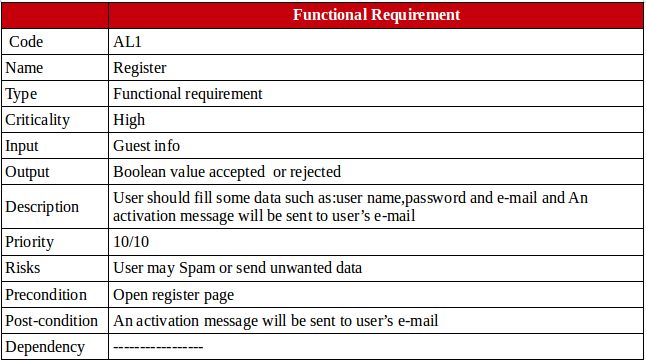
\includegraphics[scale=0.4]{./f/01}
\end{figure}

\begin{figure}[H]
\centering
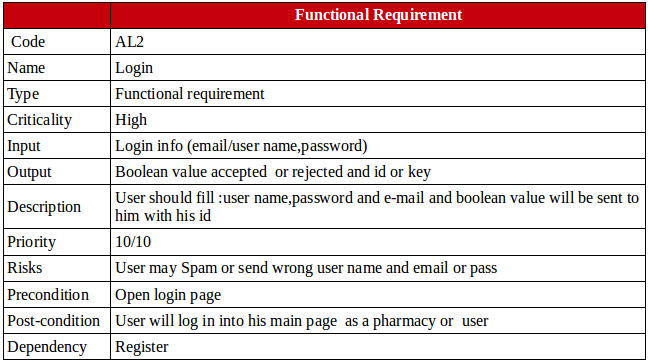
\includegraphics[scale=0.4]{./f/02}
\end{figure}

\begin{figure}[H]
\centering
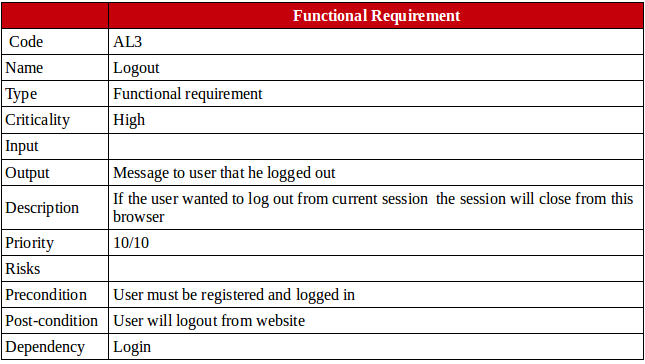
\includegraphics[scale=0.4]{./f/03}
\end{figure}

\begin{figure}[H]
\centering
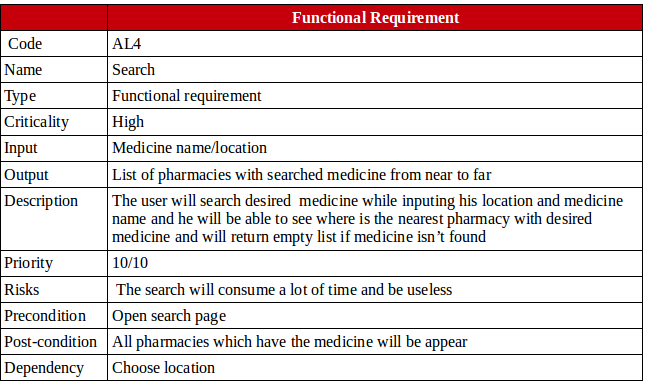
\includegraphics[scale=0.4]{./f/04}
\end{figure}

\begin{figure}[H]
\centering
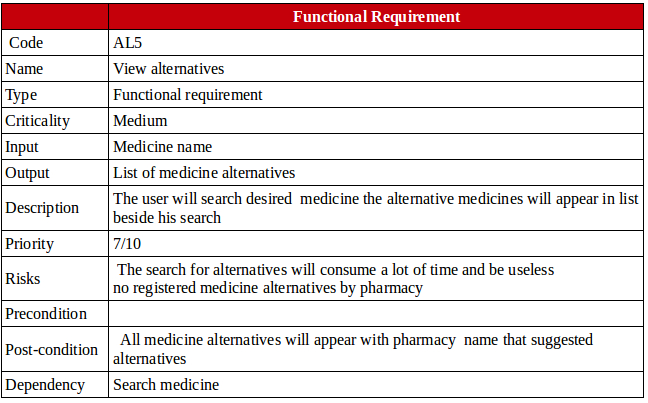
\includegraphics[scale=0.4]{./f/05}
\end{figure}

\begin{figure}[H]
\centering
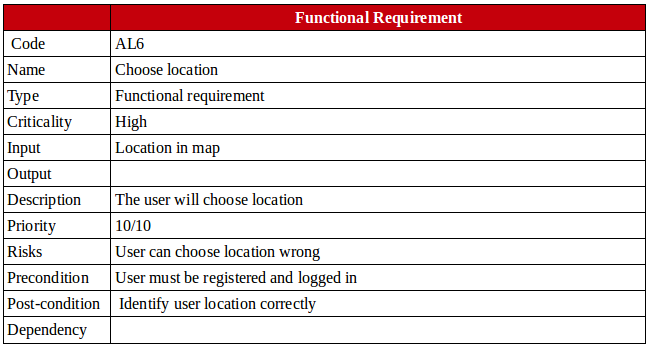
\includegraphics[scale=0.4]{./f/06}
\end{figure}

\begin{figure}[H]
\centering
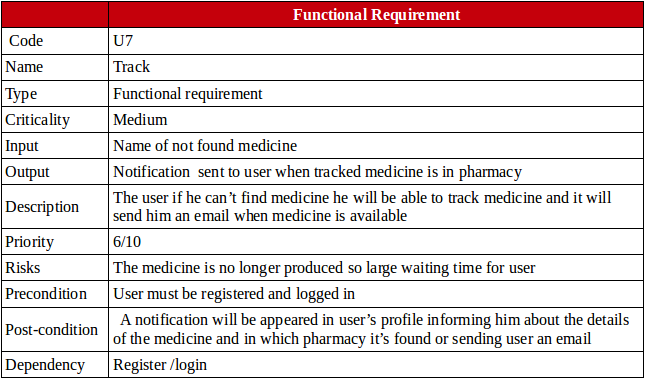
\includegraphics[scale=0.4]{./f/07}
\end{figure}

\begin{figure}[H]
\centering
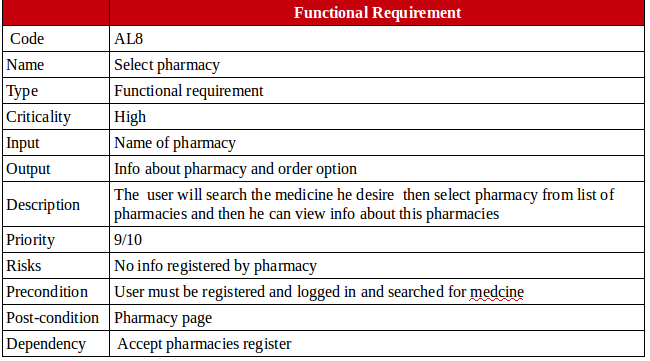
\includegraphics[scale=0.4]{./f/08}
\end{figure}

\begin{figure}[H]
\centering
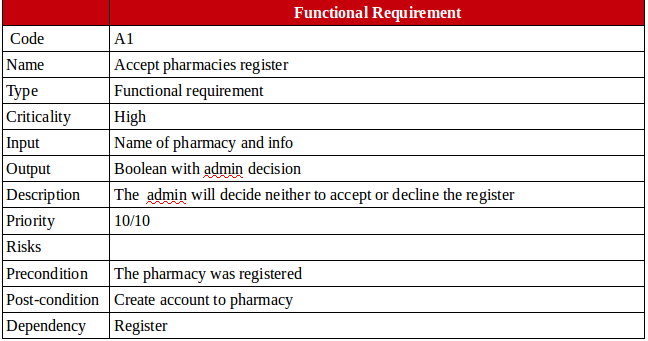
\includegraphics[scale=0.4]{./f/09}
\end{figure}

\begin{figure}[H]
\centering
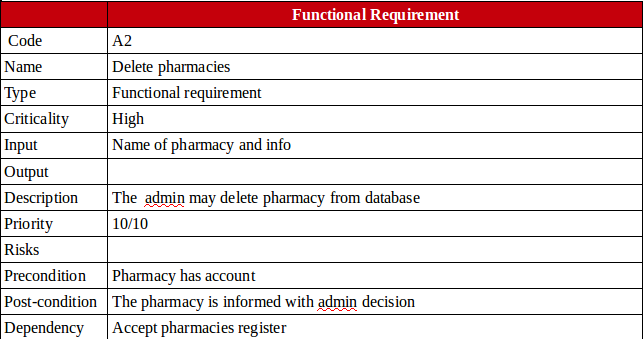
\includegraphics[scale=0.4]{./f/10}
\end{figure}

\begin{figure}[H]
\centering
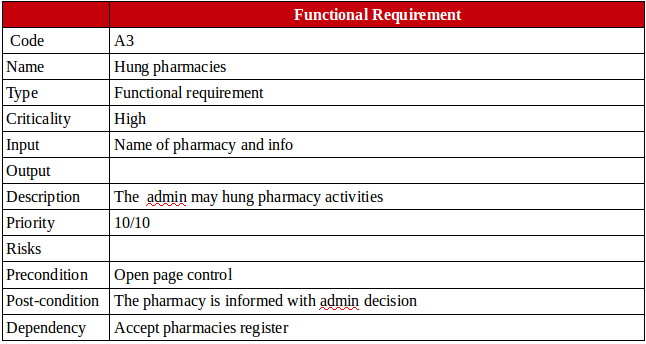
\includegraphics[scale=0.4]{./f/11}
\end{figure}

\begin{figure}[H]
\centering
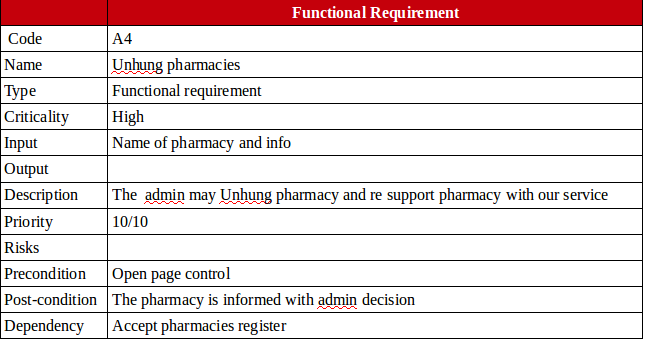
\includegraphics[scale=0.4]{./f/12}
\end{figure}

\begin{figure}[H]
\centering
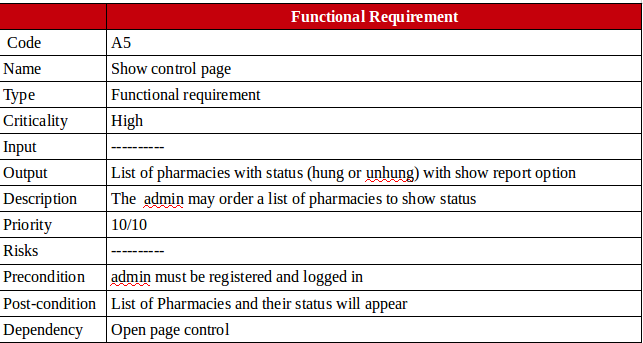
\includegraphics[scale=0.4]{./f/13}
\end{figure}

\begin{figure}[H]
\centering
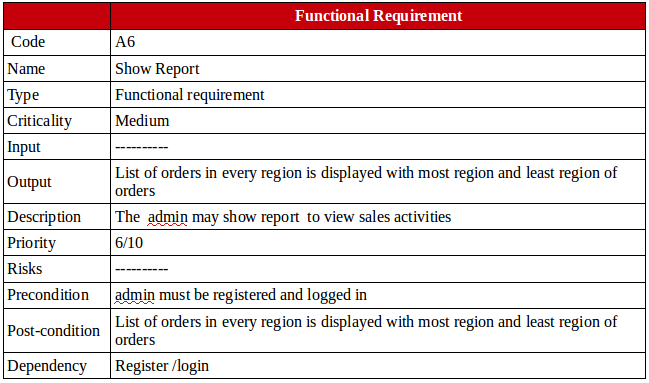
\includegraphics[scale=0.4]{./f/14}
\end{figure}

\begin{figure}[H]
\centering
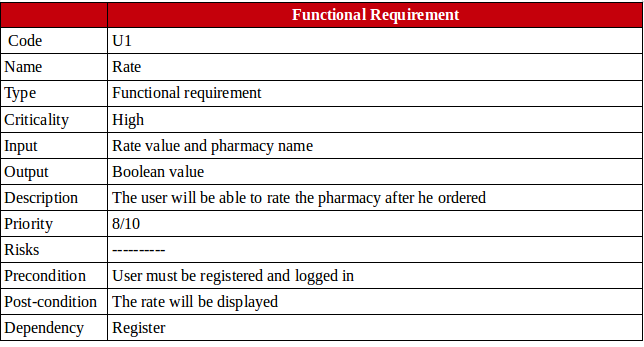
\includegraphics[scale=0.4]{./f/15}
\end{figure}

\begin{figure}[H]
\centering
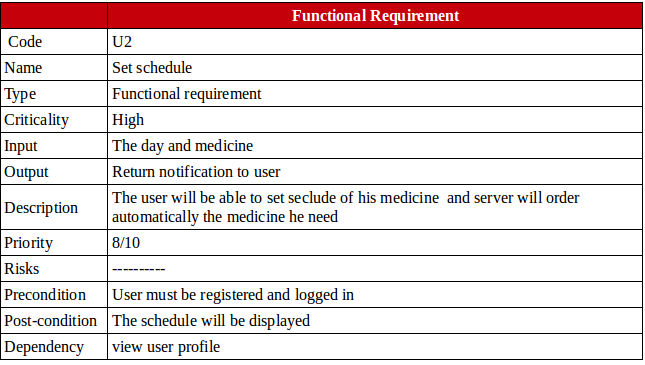
\includegraphics[scale=0.4]{./f/16}
\end{figure}

\begin{figure}[H]
\centering
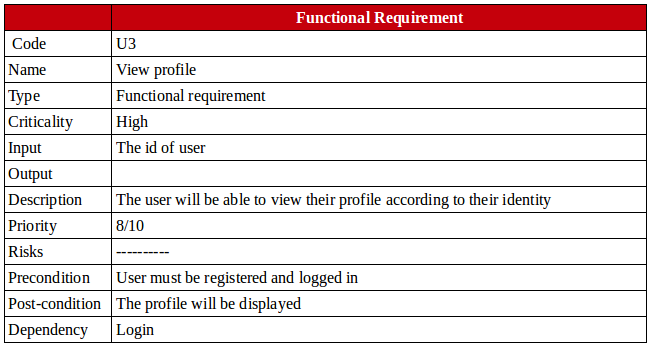
\includegraphics[scale=0.4]{./f/17}
\end{figure}

\begin{figure}[H]
\centering
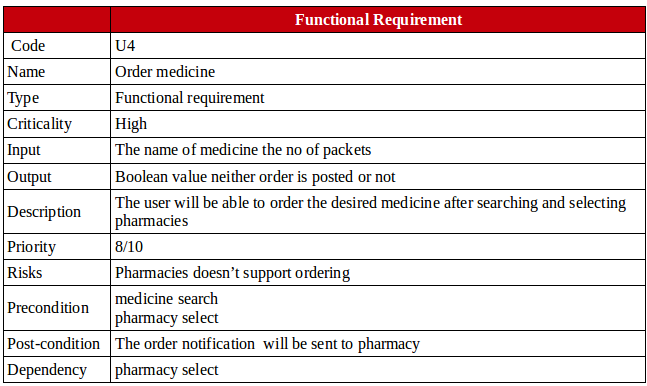
\includegraphics[scale=0.4]{./f/18}
\end{figure}

\begin{figure}[H]
\centering
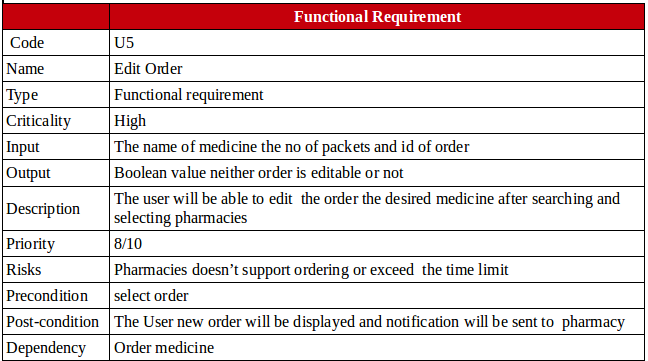
\includegraphics[scale=0.4]{./f/19}
\end{figure}

\begin{figure}[H]
\centering
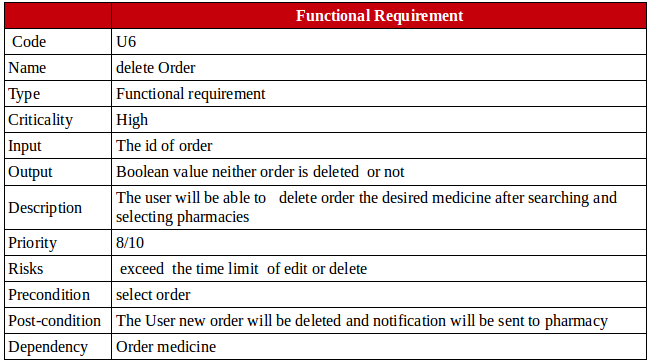
\includegraphics[scale=0.4]{./f/20}
\end{figure}

\begin{figure}[H]
\centering
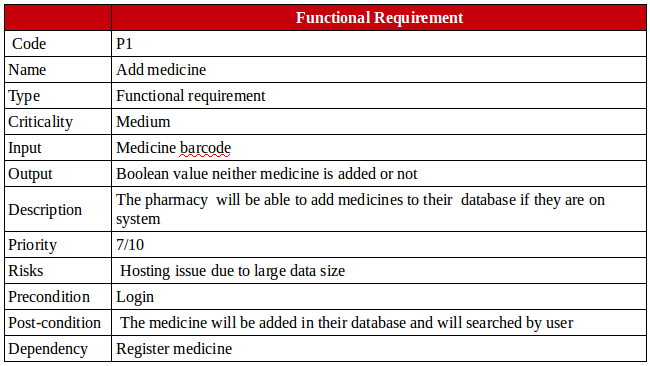
\includegraphics[scale=0.4]{./f/21}
\end{figure}

\begin{figure}[H]
\centering
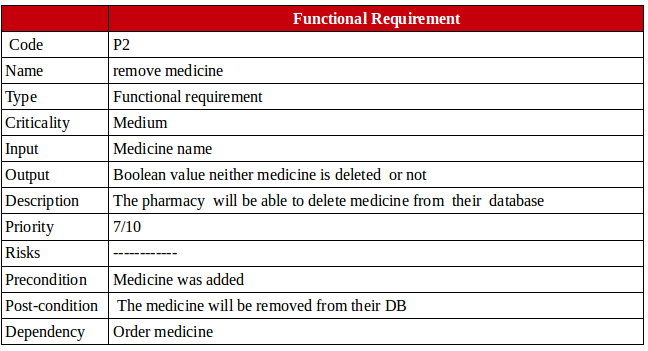
\includegraphics[scale=0.4]{./f/22}
\end{figure}

\begin{figure}[H]
\centering
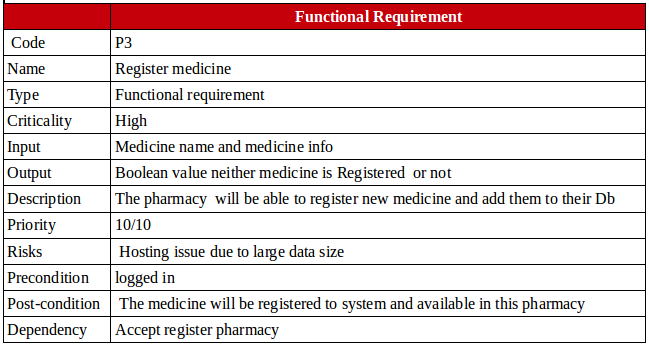
\includegraphics[scale=0.4]{./f/23}
\end{figure}

\begin{figure}[H]
\centering
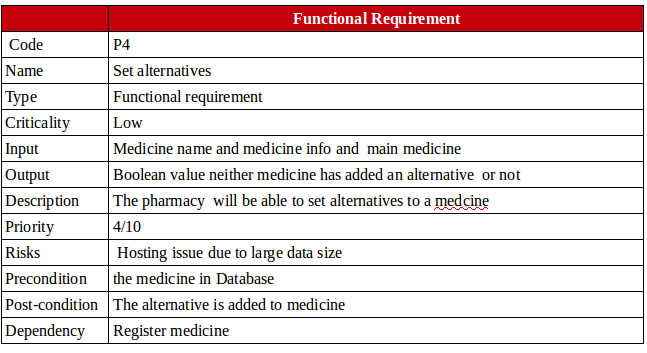
\includegraphics[scale=0.4]{./f/24}
\end{figure}

\begin{figure}[H]
\centering
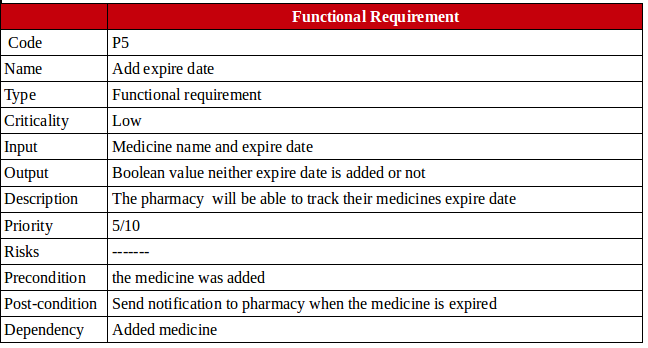
\includegraphics[scale=0.4]{./f/25}
\end{figure}

\begin{figure}[H]
\centering
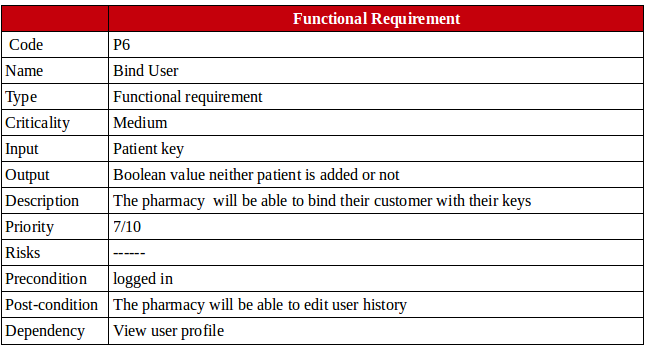
\includegraphics[scale=0.4]{./f/26}
\end{figure}

\begin{figure}[H]
\centering
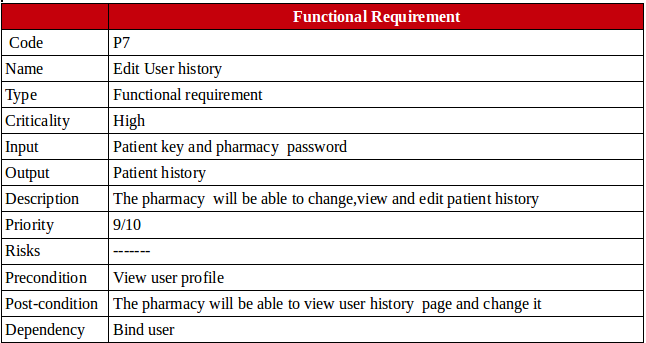
\includegraphics[scale=0.4]{./f/27}
\end{figure}

\begin{figure}[H]
\centering
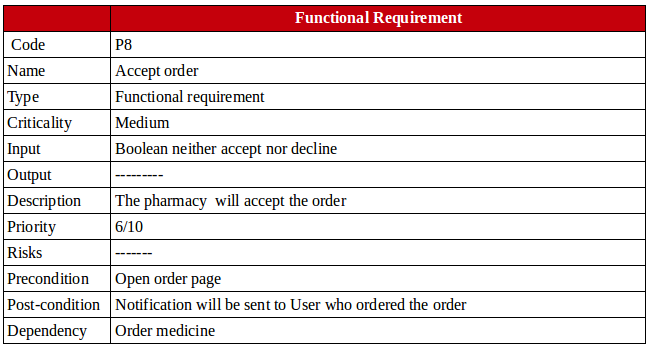
\includegraphics[scale=0.4]{./f/28}
\end{figure}

\begin{figure}[H]
\centering
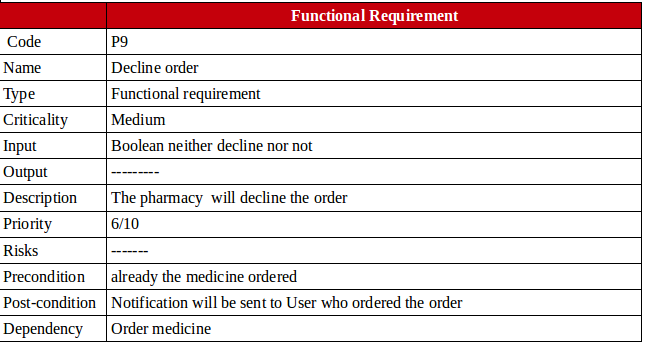
\includegraphics[scale=0.4]{./f/29}
\end{figure}

\begin{figure}[H]
\centering
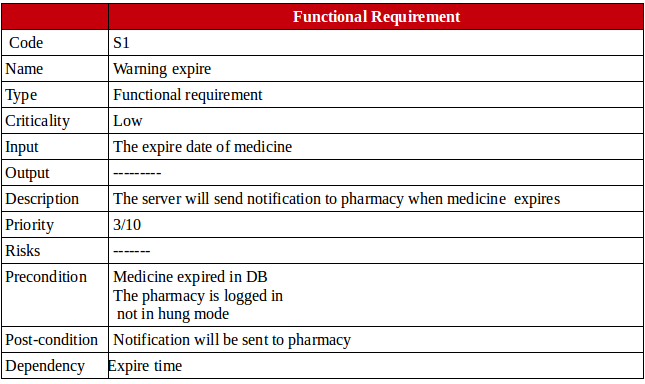
\includegraphics[scale=0.4]{./f/30}
\end{figure}

\begin{figure}[H]
\centering
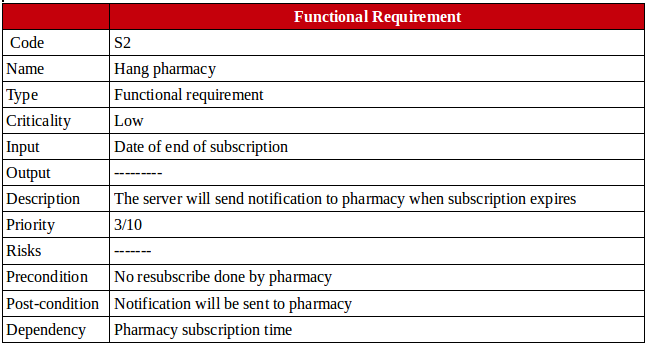
\includegraphics[scale=0.4]{./f/31}
\end{figure}

\begin{figure}[H]
\centering
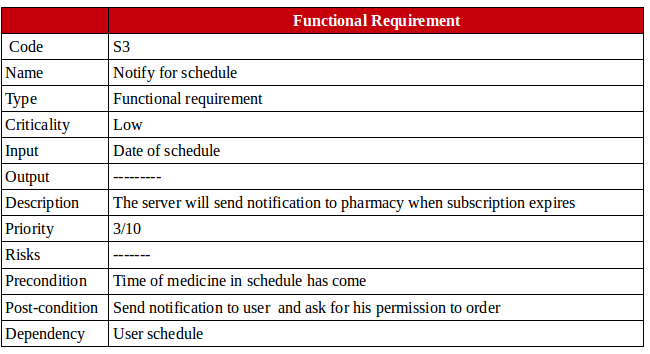
\includegraphics[scale=0.4]{./f/32}
\end{figure}


\section{Interface Requirements}
Our software will provide an API so it will provide an access for any other software development
\subsection{User Interfaces}
The interface with user will be easy and simple to insure  that he will find the medicine
\subsubsection {GUI}
This is the home page, It can navigate you to register page or to contact us, or even you can search for a desired medicine and get the nearest pharmacies that having the searched medicine.

\begin{figure}[H]
\centering
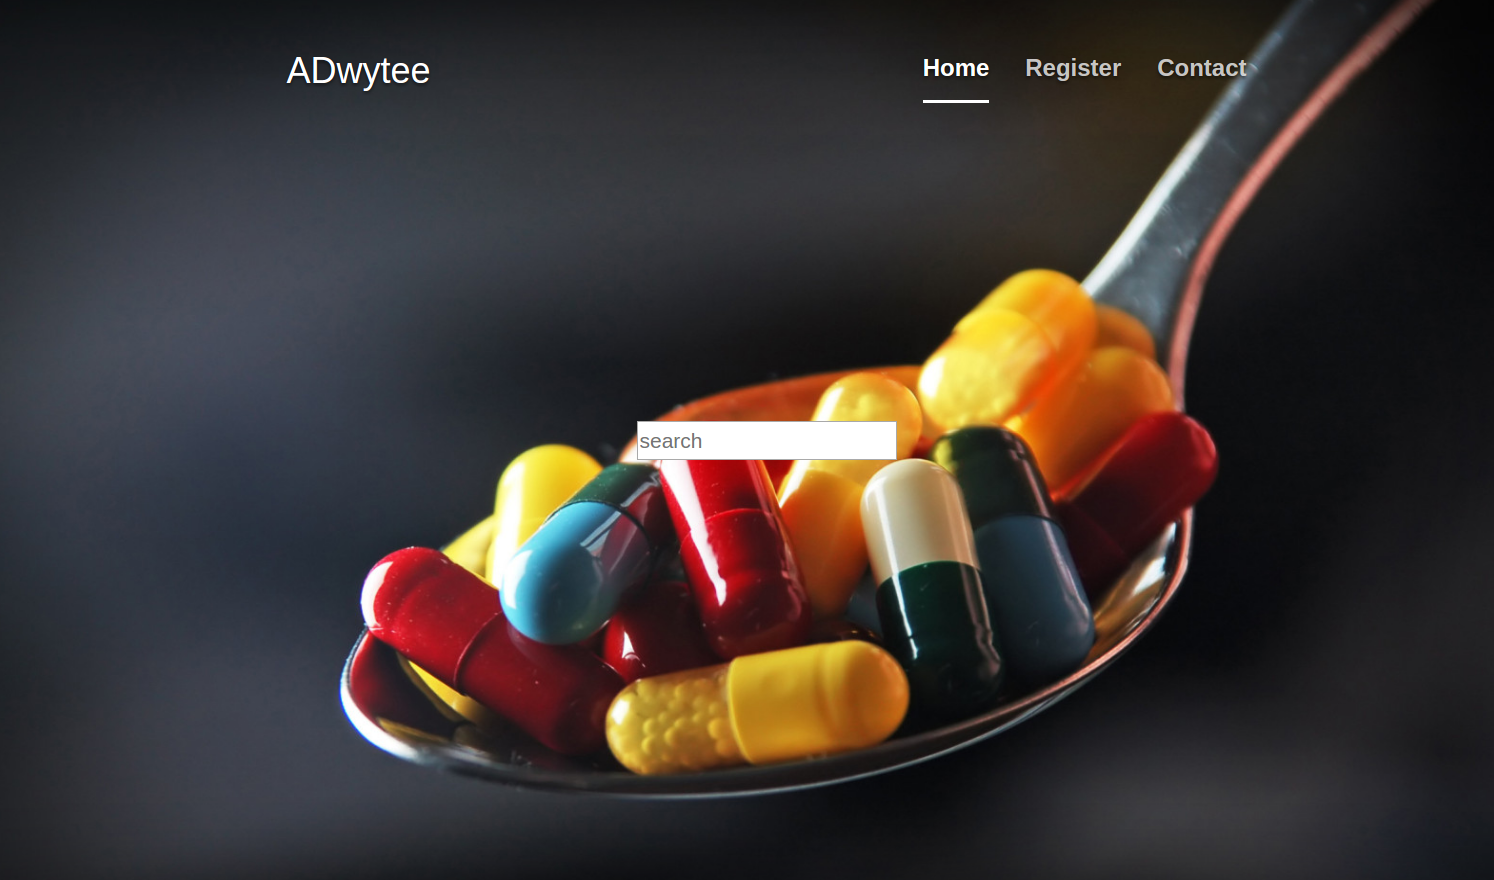
\includegraphics[scale=0.2]{./Home}
\end{figure}

\subsubsection {CLI}
...
\subsubsection {API}

\subsubsection {Diagnostics or ROM}
Apache web server

\subsection{Hardware Interfaces}
User may use Barcode reader for easier accessibility.
\subsection{Communications Interfaces}
Will mainly relay on network connection
\subsection{Software Interfaces}
... 
\section{Performance Requirements}
Provide search results with max delay 0.2 sec 
and provide the pharmacy location with the highest precision with radius of default value 2.5km.
\section{Design Constraints}
Must be easy to use interface with simple ads included.
\subsection{ Standards Compliance}
\subsection{ Hardware Limitations}
\subsection{ others as appropriate}

\section{Other non-functional attributes}

\subsection {Security}

\begin{figure}[H]
\centering
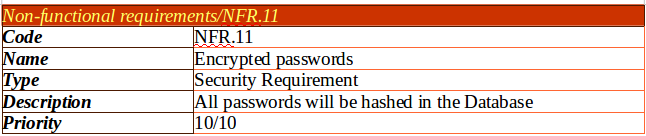
\includegraphics[scale=0.4]{./nonf/01}
\end{figure}

\subsection {Binary Compatibility}

\begin{figure}[H]
\centering
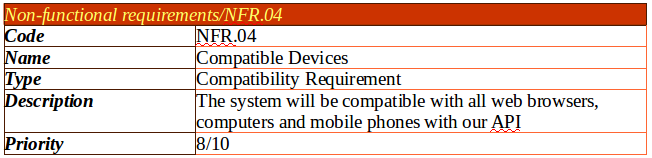
\includegraphics[scale=0.4]{./nonf/02}
\end{figure}

\subsection {Reliability}

\begin{figure}[H]
\centering
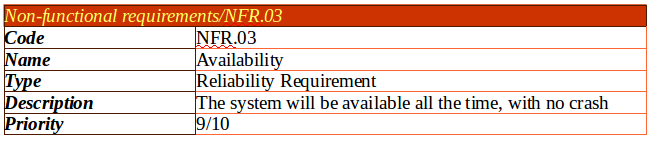
\includegraphics[scale=0.4]{./nonf/03}
\end{figure}

\subsection {Maintainability}

\begin{figure}[H]
\centering
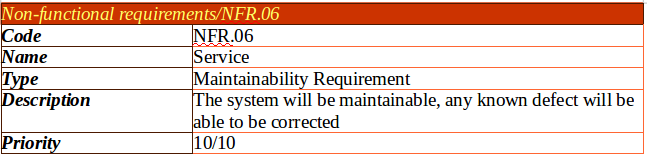
\includegraphics[scale=0.4]{./nonf/04}
\end{figure}

\subsection {Portability}

\begin{figure}[H]
\centering
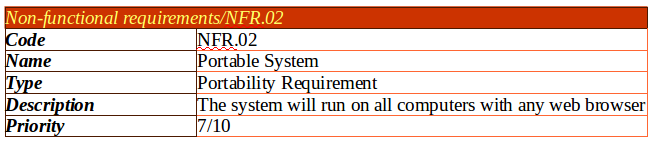
\includegraphics[scale=0.4]{./nonf/05}
\end{figure}

\subsection {Re-usability}

\begin{figure}[H]
\centering
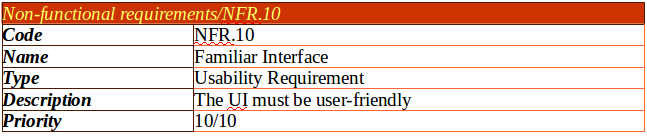
\includegraphics[scale=0.4]{./nonf/06}
\end{figure}

\subsection {Serviceability}

\begin{figure}[H]
\centering
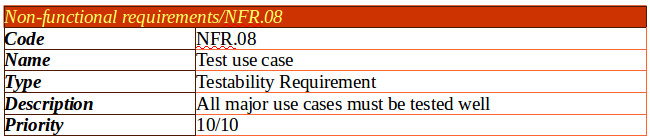
\includegraphics[scale=0.4]{./nonf/07}
\end{figure}

\subsection {others as appropriate}

\begin{figure}[H]
\centering
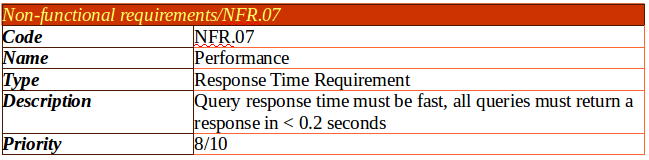
\includegraphics[scale=0.4]{./nonf/08}
\end{figure}

\begin{figure}[H]
\centering
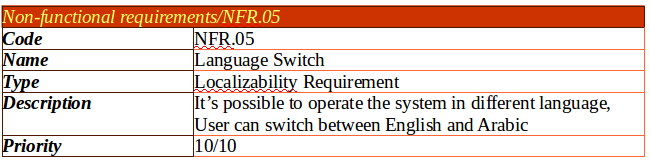
\includegraphics[scale=0.4]{./nonf/09}
\end{figure}

\begin{figure}[H]
\centering
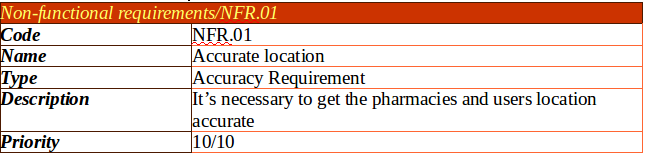
\includegraphics[scale=0.4]{./nonf/10}
\end{figure}

\begin{figure}[H]
\centering
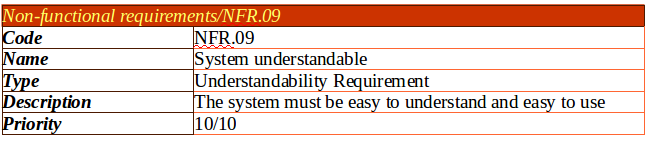
\includegraphics[scale=0.4]{./nonf/11}
\end{figure}


\section{Preliminary Object-Oriented Domain Analysis}
...
\subsection{Inheritance Relationships}
\begin{figure}[H]
\centering
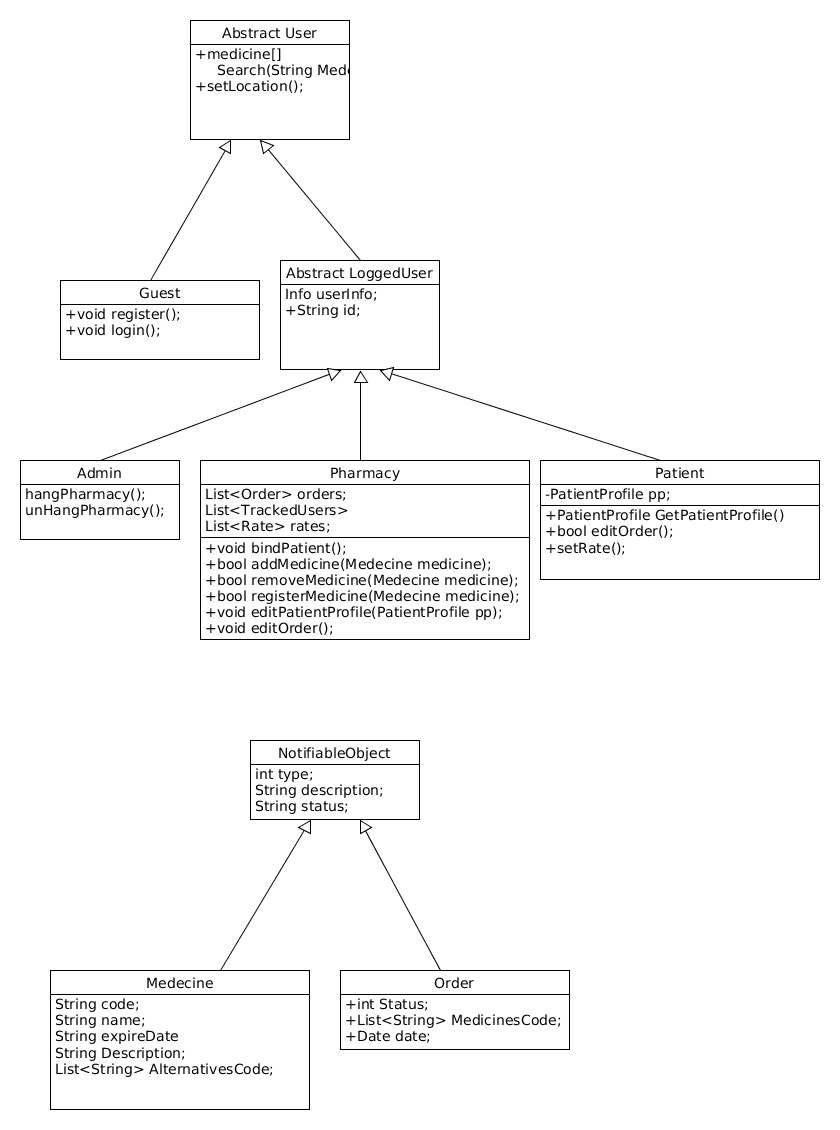
\includegraphics[scale=0.4]{./classdiagram/InhertanceRelations}
\caption{Inheritance Relations}
\end{figure}
\subsection{Class descriptions}
\begin{figure}[H]
\centering
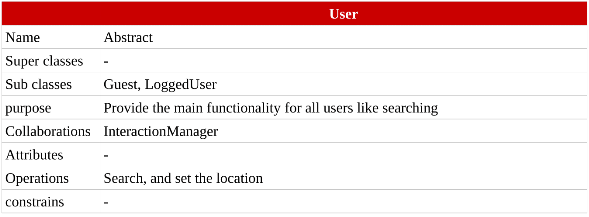
\includegraphics[scale=0.4]{./classdiagram/description/01}
\end{figure}
\begin{figure}[H]
\centering
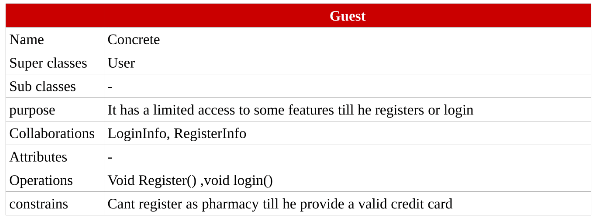
\includegraphics[scale=0.4]{./classdiagram/description/02}
\end{figure}
\begin{figure}[H]
\centering
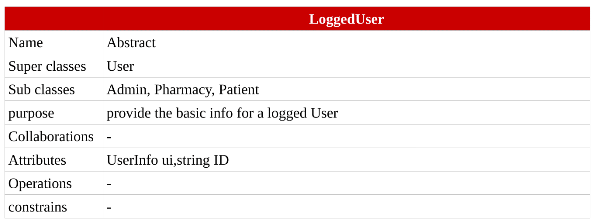
\includegraphics[scale=0.4]{./classdiagram/description/03}
\end{figure}
\begin{figure}[H]
\centering
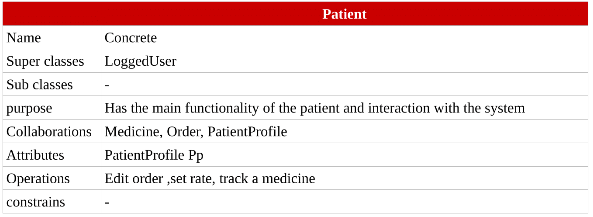
\includegraphics[scale=0.4]{./classdiagram/description/04}
\end{figure}
\begin{figure}[H]
\centering
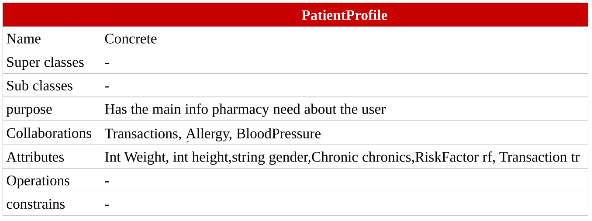
\includegraphics[scale=0.4]{./classdiagram/description/05}
\end{figure}
\begin{figure}[H]
\centering
\includegraphics[scale=0.4]{./classdiagram/description/06}
\end{figure}

\begin{figure}[H]
\centering
\includegraphics[scale=0.4]{./classdiagram/description/07}
\end{figure}

\begin{figure}[H]
\centering
\includegraphics[scale=0.4]{./classdiagram/description/08}
\end{figure}

\begin{figure}[H]
\centering
\includegraphics[scale=0.4]{./classdiagram/description/09}
\end{figure}

\begin{figure}[H]
\centering
\includegraphics[scale=0.4]{./classdiagram/description/10}
\end{figure}

\begin{figure}[H]
\centering
\includegraphics[scale=0.4]{./classdiagram/description/11}
\end{figure}

\begin{figure}[H]
\centering
\includegraphics[scale=0.4]{./classdiagram/description/12}
\end{figure}

\begin{figure}[H]
\centering
\includegraphics[scale=0.4]{./classdiagram/description/13}
\end{figure}

\begin{figure}[H]
\centering
\includegraphics[scale=0.4]{./classdiagram/description/14}
\end{figure}

\begin{figure}[H]
\centering
\includegraphics[scale=0.4]{./classdiagram/description/15}
\end{figure}

\begin{figure}[H]
\centering
\includegraphics[scale=0.4]{./classdiagram/description/16}
\end{figure}

\begin{figure}[H]
\centering
\includegraphics[scale=0.4]{./classdiagram/description/17}
\end{figure}

\begin{figure}[H]
\centering
\includegraphics[scale=0.4]{./classdiagram/description/18}
\end{figure}


\section{Operational Scenarios}

\begin{figure}[H]
\centering
\includegraphics[scale=0.4]{./scenario/01}
\end{figure}
\begin{figure}[H]
\centering
\includegraphics[scale=0.4]{./scenario/02}
\end{figure}
\begin{figure}[H]
\centering
\includegraphics[scale=0.4]{./scenario/03}
\end{figure}
\begin{figure}[H]
\centering
\includegraphics[scale=0.4]{./scenario/04}
\end{figure}
\begin{figure}[H]
\centering
\includegraphics[scale=0.4]{./scenario/05}
\end{figure}
\begin{figure}[H]
\centering
\includegraphics[scale=0.4]{./scenario/06}
\end{figure}
\begin{figure}[H]
\centering
\includegraphics[scale=0.4]{./scenario/07}
\end{figure}
\begin{figure}[H]
\centering
\includegraphics[scale=0.4]{./scenario/08}
\end{figure}
\begin{figure}[H]
\centering
\includegraphics[scale=0.4]{./scenario/09}
\end{figure}
\begin{figure}[H]
\centering
\includegraphics[scale=0.4]{./scenario/10}
\end{figure}
\begin{figure}[H]
\centering
\includegraphics[scale=0.4]{./scenario/11}
\end{figure}
\begin{figure}[H]
\centering
\includegraphics[scale=0.4]{./scenario/12}
\end{figure}
\begin{figure}[H]
\centering
\includegraphics[scale=0.4]{./scenario/13}
\end{figure}
\begin{figure}[H]
\centering
\includegraphics[scale=0.4]{./scenario/14}
\end{figure}
\begin{figure}[H]
\centering
\includegraphics[scale=0.4]{./scenario/15}
\end{figure}
\begin{figure}[H]
\centering
\includegraphics[scale=0.4]{./scenario/16}
\end{figure}
\begin{figure}[H]
\centering
\includegraphics[scale=0.4]{./scenario/17}
\end{figure}
\begin{figure}[H]
\centering
\includegraphics[scale=0.4]{./scenario/18}
\end{figure}
\begin{figure}[H]
\centering
\includegraphics[scale=0.4]{./scenario/19}
\end{figure}
\begin{figure}[H]
\centering
\includegraphics[scale=0.4]{./scenario/20}
\end{figure}
\begin{figure}[H]
\centering
\includegraphics[scale=0.4]{./scenario/21}
\end{figure}
\begin{figure}[H]
\centering
\includegraphics[scale=0.4]{./scenario/22}
\end{figure}
\begin{figure}[H]
\centering
\includegraphics[scale=0.4]{./scenario/23}
\end{figure}
\begin{figure}[H]
\centering
\includegraphics[scale=0.4]{./scenario/24}
\end{figure}
\begin{figure}[H]
\centering
\includegraphics[scale=0.4]{./scenario/25}
\end{figure}
\begin{figure}[H]
\centering
\includegraphics[scale=0.4]{./scenario/26}
\end{figure}
\begin{figure}[H]
\centering
\includegraphics[scale=0.4]{./scenario/27}
\end{figure}
\begin{figure}[H]
\centering
\includegraphics[scale=0.4]{./scenario/28}
\end{figure}
\begin{figure}[H]
\centering
\includegraphics[scale=0.4]{./scenario/29}
\end{figure}
\begin{figure}[H]
\centering
\includegraphics[scale=0.4]{./scenario/30}
\end{figure}
\begin{figure}[H]
\centering
\includegraphics[scale=0.4]{./scenario/31}
\end{figure}
\begin{figure}[H]
\centering
\includegraphics[scale=0.4]{./scenario/32}
\end{figure}
\begin{figure}[H]
\centering
\includegraphics[scale=0.4]{./scenario/01}
\end{figure}


\section{Preliminary Schedule Adjusted}
... 
\section{Preliminary Budget Adjusted}
... 
\section{Appendices}
... 
\subsection{Definitions, Acronyms, Abbreviations}
... 
\subsection{Collected material}

\section {References}
\bibliographystyle{IEEEtranS}

\bibliography{dissertationbib}

\end{document}